\documentclass[UTF8]{article}
\usepackage{amsmath}
\usepackage{booktabs}
\usepackage{graphicx}
\usepackage{enumerate}
\usepackage{caption}
\usepackage{subfig}



\title{Understanding Clouds from Satellite Images}
\author{Lijin Zhou, WenBo Cao, Bowen Li}


\begin{document}


\maketitle

Github repoitory: https://github.com/Mulburry0v0/CS583FinalProject

\section{Introduction}
Climate change has been at the top of our minds and on the forefront of important political decision-making for many years. Shallow clouds play a huge role in determining the Earth's climate. They’re also difficult to understand and to represent in climate models. By classifying different types of cloud organization, improving physical understanding of these clouds, which in turn will help scientists build better climate models. In this competition, we are required to use the dataset they provided to help demystify an important climatic variable. 

\section{Related work}
We all know about the image classification problem. We can solve it with ConvNets and Transfer Learning using pre-trained nets. However, there are some other problems which are more complex. Theses problems can be divided into 4 major buckets: semantic segmentation, classification and localization, object detection and instance segmentation. This challenge is a task combining object detection and instance segmentation, which is important, popular but much harder. \par
\noindent Our work is inspired by a fully convolutional network, with both long and short skip connections which is published in 2016 DLMIA. The purpose of this method is to have biomedical image segmentation. They have constructed a model based on U-Net with ResNet, which shows its effectiveness by analyzing the weights within the network. Since our tasks are similar, we decided to use U-Nets and ResNets based models predicting on auto collaborated data. After firstly training the dataset with basic features analysis, we build three models which are U-Net, U-Net with EfficientNet and U-Net with ResNet. With the comparison of these three architecture, which method is more effective in this competetion will show.
 



\section{Solution}
\subsection{Dataset Description}
	\begin{itemize}
		\item train.csv: the run length encoded segmentations for each image-label pair in the train\_images
		\item train\_images.zip: folder of training images
		\item test\_images.zip: folder of test images; our task is to predict the segmentations masks of each of the 4 cloud types (labes) for each image.
	\end{itemize}
In this competition, we are asked to identify regions in satellite images that contain certain cloud formations, with label name: Fish, Flower, Gravel, Sugar. For each image in the test set, we must segment the regions of each cloud formation label. Each image has at least one cloud formation, and can possibly contain up to all four.\par
\noindent The images are downloaded from NASA Worldview. Three regions spanning 21 degrees longitude and 14 degrees latitude, were chosen. The labels were created in a crowd-sourcing activity which has a team of 68 scientists identified areas of cloud patterns in each image, and each images was labeled by approximately 3 different scientists. \par
\noindent The segment for each cloud formation label for an image is encoded into a single row, even if there are several non-contiguous areas of the same formation in an image. 

\subsection{Evaluation Method}
This competition is evaluated on the team Dice coefficient. The Dice coefficient can be used to compare the pixel-wise agreement between a predicted segmentation and its corresponding ground truth. The formula is given by:
	\begin{displaymath}
	\frac{2*|X\bigcap Y|}{|X|+|Y|}
	\end{displaymath}
where X is  the predicted set of pixels and Y is the ground truth. The Dice coefficient is defined to be 1 where both X and Y are empty.
\subsection{Models}
	\subsubsection{Baseline and Feature Engineered Model}
	\begin{enumerate}
		\item U-Net\par
		\noindent U-Net was first designed especially for medical image segmentation. The architecture looks like a ‘U’ which justifies its name. Unlike CNN only convert the image into the feature mapping which used further for classification, U-Net will meanwhile convert the feature mapping to the image. Doing so will make preserve the structural integrity of the image which would reduce distortion enormously.\par
		\begin{figure}[h]
			\centering
			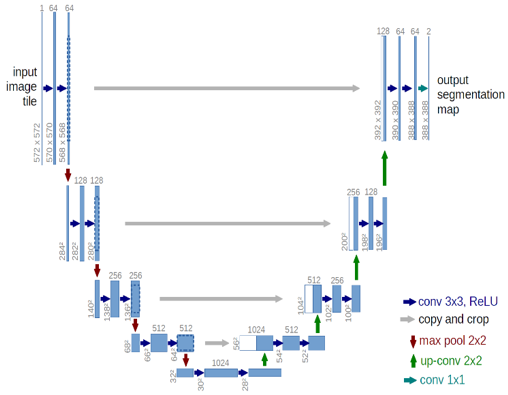
\includegraphics[width=8cm]{1.png}
			\caption{U-Net}
		\end{figure}
		\noindent This architecture consists of three sections: The contraction, The bottleneck, and the expansion section. The heart of this architecture lies in the expansion section. Each block passes the input to two 3X3 CNN layers followed by a 2X2 up-sampling layer. Although next block get half to maintain symmetry because of 2X2 up-sampling layer, every time the input is also get appended by feature maps of the corresponding contraction layer. That means previous feature mapping will be combined with maintain symmetry from last layer to reconstructed image. That’s why U-Net have good performance in Instance segmentation task.
		
		\item U-Net with EfficientNet\par
		\noindent In this method, we implemented Unet with EfficientNet as encoder.\par
		
		\noindent EfficientNets are a family of image classification models, which achieve state-of-the-art accuracy, yet being an order-of-magnitude smaller and faster than previous models. EfficientNets based on AutoML and Compound Scaling. In particular, they first use AutoML MNAS Mobile framework to develop a mobile-size baseline network, named as EfficientNet-B0; Then, they use the compound scaling method to scale up this baseline to obtain EfficientNet-B1 to B7.\par
		\begin{figure}[h]
			\centering
			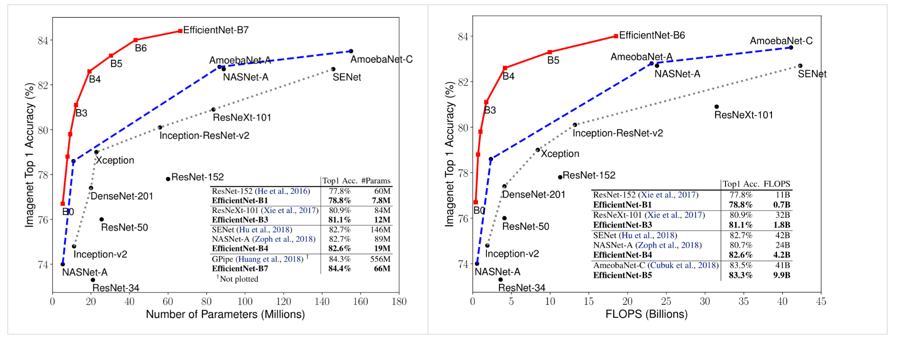
\includegraphics[width=10cm]{2.png}
			\caption{U-Net with EfficientNet}
		\end{figure}
		\noindent EfficientNets achieve state-of-the-art accuracy on ImageNet with an order of magnitude better efficiency:
		\begin{itemize}
			\item In high-accuracy regime, EfficientNet-B7 achieves state-of-the-art 84.4\% top-1 / 97.1\% top-5 accuracy on ImageNet with 66M parameters and 37B FLOPS, being 8.4x smaller and 6.1x faster on CPU inference than previous best Gpipe.
			\item In middle-accuracy regime, EfficientNet-B1 is 7.6x smaller and 5.7x faster on CPU inference than ResNet-152, with similar ImageNet accuracy.
			\item •	Compared with the widely used ResNet-50, EfficientNet-B4 improves the top-1 accuracy from 76.3\% of ResNet-50 to 82.6\% (+6.3\%), under similar FLOPS constraint.
		\end{itemize}
		\item U-Net with ResNet\par
		\noindent ResNet is a CNN architecture, made up of series of residual blocks (ResBlocks) with skip connections differenting ResNets from other CNNs. The networks skip connections can create a flatter loss surface which is much easier for the model to be trained with optimal weights.\par
		\begin{figure}[htbp]
		\centering
		\subfloat[Loss \& Val Loss]{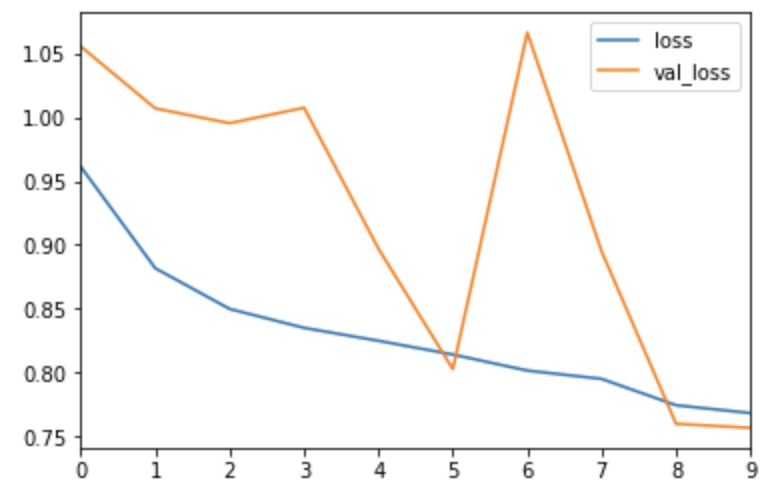
\includegraphics[height=4cm,width=5.5cm]{3.png}}
		\subfloat[Dice Coef \& Val Dice Coef]{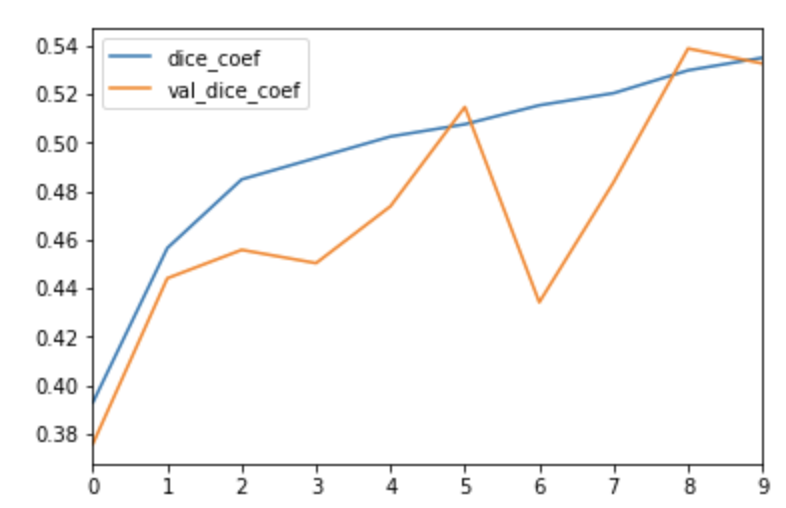
\includegraphics[height=4cm,width=5.5cm]{4.png}}
		\caption{U-Net with ResNet}
		\label{fig}
		\end{figure}
		\noindent As we mentioned above, U-Nets are very good for creating segmentation masks and for image processing. However, when using only a U-Net architecture the predictions tend to lack fine details, to help address this cross or skip connections can be added between blocks of the network. In our models, we have used a ResNet-18 for the encoder and decoder, a 18 layer ResNet architecture, as this has been found to be very effective by experiments. So the baseline is a U-Nets with ResNet-18 Encoders and cross connections.
		

	\end{enumerate}
	\subsubsection{Optimization}
	\begin{enumerate}
		\item Adam with Gradient Accumulation\par
		\noindent When we are working on this memory-demanding algorithm for segmentation, we want to accumulate the gradients during training, meaning that the weights of the model are not updated after every single batch. The gradients from each batch are accumulated and then averaged for a single weight-update action. The reason is that “Colab” only have 12GB RAM available and sometime too much memory consumption will kill our model.\par
		\noindent When we implement Gradient Accumulation, gradient will be update after some certain steps (e.g. if we set batch\_size = 32 and accumulation\_step = 8, gradient will be updated at the 256th iteration. We have three advantages of Gradient Accumulation
		\begin{enumerate}
			\item Reducing memory consumption by accumulating gradients
			\item Alleviating the bad influence caused by some noisy gradients by performing average operation
		\end{enumerate}
		\item Post-Processing Segmentation\par
		\noindent To improve the performance based on EfficientUnet, we created a classifier to distinguish types of cloud formations. Using this classifier, we’d check if it improves currently. The process is listed below:\par
		\begin{enumerate}
			\item [(1)] PR-AUC-Based Callback
			\begin{itemize}
				\item to estimate AUC under precision recall curve for each class
				\item to early stop after 5 epochs of no improvement in mean PR AUC
				\item save a model with the best PR AUC in validation
				\item to reduce learnint rate on PR AUC plateau
				\end{itemize}
			\item [(2)] Classifier: DenseNet169
			\item [(3)] Selecting post-processing thresholds through PR-AUC curves
			\item [(4)] Do the post-processing segmentation
			\item [(5)] Final output improves about 0.02
		\end{enumerate}
		\item Test Time Augmentation\par
		\noindent Test time augmentation is a common way to improve the accuracy of image classifiers especially in the case of deep learning. The intuition behind this is that even if the test image is not too easy to make a prediction, the transformations change it such that the model has higher chances of capturing the target shape and predicting accordingly.\par
		\noindent We set threshold to remove small masks and add TTA wrapper on our trained model and use the wrapped model to predict on the test images. With TTA wrapper, the prediction of the ResUNet model improves as much as 0.07, which is a huge increasement.
		\item Gamma Correction\par
		\noindent Gamma encoding of images is used to optimize the usage of bits when encoding an image, or bandwidth used to transport an image, by taking advantage of the non-linear manner in which humans perceive light and color. In order to get more accurate prediction, we add gamma correction in the data generator.
		\item Blending Mask\par
		\noindent Blending mask opens up opportunity for diversity in the representational capacity of the model. They are a very common enhancement to traditional machine learning models. We try blending three best submissions and the result shows that it does have an improvement.\par
	\end{enumerate}

	\subsubsection{Comparison}
		\begin{table}[h]
	\centering
	\setlength{\abovecaptionskip}{0pt}    
	\setlength{\belowcaptionskip}{10pt}
	\caption{Mean of the Dice coefficients}
	\begin{tabular}{lc}
	\toprule
	Model& Dice coefficients\\
	\midrule
	U-Net& 0.5013\\
	U-Net \& EfficientNet& 0.4365\\
	U-Net \& EfficientNet(Post Processing Segmentation) & 0.4515\\
	U-Net \& ResNet& 0.5971\\
	U-Net \& ResNet(AdamAccumulation,TTA, gamma correction) & 0.6534\\
	Blending Mask&  0.6537\\
	\bottomrule
	\end{tabular}
	\end{table}
\subsection{Kaggle score and rank}
According to our best private score 0.6537, our rank is 853, about 55\% on the leaderborad.
 
\section{Conclusion}
Our project is to help build a model that can perform nearly like human eyes, which are really good at detecting features. In this way, we can help scientists better understand how clouds will shape our future climate and guide the development of next-generation models which could reduce uncertainties in climate projections. The murky boundaries between different forms of organization of clouds are the major sticking points. To get over these difficulties, we have read lots of articles and tried several method, including U-Net, U-Net with EfficientNets, U-Net with ResNets. According to the result of comparison, we finally found a model which performed well.\par
\noindent By using Adam gradient accumulation, post-processing segmentation, TTA, Gamma Correction and blending mask, we have achieved a significant improvement over the baseline models. And among these three models, U-Net with ResNet Encoders and cross connections performs the best. But there is still a gap between our model and some excellent model on Kaggle. Their performance could get 0.68. Our future task is to try some more methods and keep updating our models to get better prediction. \par
\section{Future Work}
\begin{enumerate}
		\item Estimate distribution of classes in test set using the classifier. Then, if necessary and doable, modify validation set accordingly
		\item Use the classifier with explainability technique Gradient-weighted Class Activation Mapping to generate a baseline, (please see GradCAM: extracting masks from classifier 
		\item Improve the classifier, use the classifier as backbone for UNet-like solution
\end{enumerate}

\begin{thebibliography}{8}
\bibitem{} Vadivel, Shamik Sural, A.K.M., 2005. Human color perception in the hsv space and its application in histogram generation for image retrieval. URL: https://doi.org/10.1117/12.586823, doi:10.1117/12.586823.
\bibitem{} Audebert, N., Le Saux, B., Lefe`vre, S., 2018. Beyond rgb: Very high resolution urban remote sensing with multimodal deep networks. ISPRS Journal of Photogrammetry and Remote Sensing 140, 20–32.
\bibitem{} Audebert, N., Le Saux, B., Lefvre, S., 2017. Segment-before-detect: Vehicle detection and classification through semantic segmentation of aerial images. Remote Sensing 9. URL: http://www.mdpi.com/2072-4292/9/4/368, doi:10.3390/rs9040368.
\bibitem{} Foivos I. Diakogiannis, Francois Waldner, Peter Caccetta, Chen Wu., 2019. ResUNet-a: a deep learning framework for semantic segmentation of remotely sensed data.
\bibitem https://medium.com/huggingface/training-larger-batches-practical-tips-on-1-gpu-multi-gpu-distributed-setups-ec88c3e51255
https://www.kaggle.com/c/understanding\_cloud\_organization/discussion/105614\#latest-662360
\bibitem{} https://towardsdatascience.com/u-net-b229b32b4a71
\bibitem{} https://www.kaggle.com/xhlulu/satellite-clouds-u-net-with-resnet-encoder
\bibitem{} https://www.kaggle.com/gogo827jz/blending-submissions-using-np-logical-or\#Blending
\bibitem{} https://www.kaggle.com/cdeotte/without-ensemble-lb-0-665
\bibitem{} https://www.kaggle.com/samusram/cloud-classifier-for-post-processing/data
\bibitem{} https://www.kaggle.com/paulorzp/rle-functions-run-lenght-encode-decode
\bibitem{} https://lars76.github.io/neural-networks/object-detection/losses-for-segmentation/
\bibitem{} https://www.kaggle.com/artgor/segmentation-in-pytorch-using-convenient-tools
\end{thebibliography}



\end{document}